\documentclass[sigplan]{acmart}

\usepackage{xspace}
\usepackage{amssymb}
\usepackage{amsmath}
\usepackage{mathtools}
\usepackage{listings}
%% \usepackage[final]{graphicx}

% Copyright
%\setcopyright{none}
%\setcopyright{acmcopyright}
%\setcopyright{acmlicensed}
%\setcopyright{rightsretained}
%\setcopyright{usgov}
%\setcopyright{usgovmixed}
%\setcopyright{cagov}
%\setcopyright{cagovmixed}


% DOI
%\acmDOI{10.475/123_4}
%
%% ISBN
%\acmISBN{123-4567-24-567/08/06}
%
%%Conference
\acmConference[TyDe'17]{}{September 2017}{Oxford, United Kingdom}
%\acmYear{1997}
%\copyrightyear{2016}

%\acmPrice{15.00}

\lstdefinelanguage{Encore}
{
  numbers=left,
  %% frame=single,
  literate={~~>}{$\leadsto\ $}{2} {liftf}{$^\circ$}{1} {liftfp}{$^\dagger$}{1},
  basicstyle=\fontsize{8.5}{10}\selectfont\tt\color{black},
  aboveskip=1ex,
  belowskip=1ex,
  mathescape=true,
  tabsize=2,
  columns=fullflexible,
  xleftmargin=4ex,
  resetmargins=true,
  showstringspaces=false,
  morecomment=[l]{--},
  morecomment=[s]{/*}{*/},
  escapeinside=??,
  morekeywords={async,finish,get,await,def,passive,active,void,this,class,fun,
                string,uint,int,real,bool,Fut,Par,end,let,in,var,val,then,lin,read}
}

\newcommand{\TODO}[1]{\textcolor{red}{\textbf{[#1]}}}

\begin{document}
\title{Extended Abstract: Affine killing}
\subtitle{Semantics for stopping the ParT}

\author{Kiko Fernandez-Reyes}
\orcid{0000-0001-8654-118X}
\affiliation{%
  \institution{Uppsala University}
  \streetaddress{}
  %% \city{Uppsala}
}
\email{kiko.fernandez@it.uu.se}

\author{Dave Clarke}
\affiliation{%
  \institution{Uppsala University}
  %% \city{Uppsala}
}
\email{dave.clarke@it.uu.se}


\begin{abstract}
Speculative, parallel abstractions allow that, once a result is computed,
the remaining (unnecessary) speculative computations can be safely stopped.
%
However, it is difficult to know when it is safe to stop an ongoing computation.
%
This paper presents a refinement of the parallel speculative
ParT abstraction~\cite{DBLP:conf/coordination/Fernandez-Reyes16}
with an affine type system that allows \emph{in-place updates},
and \textit{killing} speculative computations using \emph{thread-local reasoning}.
There is ongoing work to prove the soundness of the calculus
and implement it in the Encore language~\cite{DBLP:conf/sfm/BrandauerCCFJPT15}.
\end{abstract}

%
% The code below should be generated by the tool at
% http://dl.acm.org/ccs.cfm
% Please copy and paste the code instead of the example below.
%
\begin{CCSXML}
<ccs2012>
<concept>
<concept_id>10003752.10010124.10010125.10010127</concept_id>
<concept_desc>Theory of computation~Functional constructs</concept_desc>
<concept_significance>500</concept_significance>
</concept>
<concept>
<concept_id>10003752.10010124.10010125.10010130</concept_id>
<concept_desc>Theory of computation~Type structures</concept_desc>
<concept_significance>500</concept_significance>
</concept>
<concept>
<concept_id>10003752.10003753.10003761.10003762</concept_id>
<concept_desc>Theory of computation~Parallel computing models</concept_desc>
<concept_significance>300</concept_significance>
</concept>
<concept>
<concept_id>10003752.10003790.10011740</concept_id>
<concept_desc>Theory of computation~Type theory</concept_desc>
<concept_significance>300</concept_significance>
</concept>
</ccs2012>
\end{CCSXML}

\ccsdesc[500]{Theory of computation~Functional constructs}
\ccsdesc[500]{Theory of computation~Type structures}
\ccsdesc[300]{Theory of computation~Parallel computing models}
\ccsdesc[300]{Theory of computation~Type theory}


\newcommand{\Upscale}{\textsc{UpScale}\xspace}
\newcommand{\parT}{ParT\xspace}
\newcommand{\parTs}{ParTs\xspace}

\newcommand{\TT}[1]{\atask{g}{E[#1]}}
\newcommand{\typePar}[1]{\ensuremath{\mathit{Par}[#1]}}
\newcommand{\typeFut}[1]{\ensuremath{\mathit{Fut}[#1]}}
\newcommand{\typeMaybe}[1]{\ensuremath{\mathit{Maybe}[#1]}}
\newcommand{\singlePar}[1]{\ensuremath{\{#1\}}}
\newcommand{\prunesymbol}[0]{\ensuremath{\ll }}
\newcommand{\prunen}[3]{\ensuremath{#2 \prunesymbol_{#1} #3}}
\newcommand{\single}[1]{\ensuremath{\{ #1 \}}}
\newcommand{\parrn}[3]{\ensuremath{#2 \,||_{#1}\, #3}}
\newcommand{\parrnl}[4]{\ensuremath{#3 \,||^{#1}_{#2}\, #4}}
\newcommand{\bind}[2]{\ensuremath{#1 \gg\!\!= #2}}
\newcommand{\lin}[1]{\ensuremath{\texttt{lin}\ #1}}
\newcommand{\un}[1]{\ensuremath{\texttt{read}\ #1}}
\newcommand{\sub}[0]{\ensuremath{<:}}
%
\newcommand{\mode}[0]{\modekw{} \ }
\newcommand{\moden}[1]{\ensuremath{\modekw{}_{#1} \ }}
\newcommand{\modekw}[0]{\ensuremath{\kappa}}
\newcommand{\modekwn}[1]{\ensuremath{\kappa}_{#1} }
\newcommand{\e}[0]{\hookrightarrow}

\newcommand{\peekkw}{\texttt{peek}}
\newcommand{\apoison}[1]{\ensuremath{(\texttt{kill} \; #1)}}
\newcommand{\atask}[2]{\ensuremath{(\texttt{task}_{#1}\ #2)}}
\newcommand{\sfut}[1]{\ensuremath{(\texttt{fut}_{#1})}}  % single future\
\newcommand{\afut}[2]{\ensuremath{(\texttt{fut}_{#1}\ #2)}}  % future with value
\newcommand{\peekn}[3]{\ensuremath{\peekkw^{#2}_{#1}\ #3}}
\newcommand{\poisoningStates}[0]{\ensuremath{\pi}}
\newcommand{\peeksn}[2]{\ensuremath{\peekkw^{\poisoningStates}_{#1}\ #2}}

\thanks{Partly funded by the EU project FP7-612985 \Upscale: From Inherent Concurrency
    to Massive Parallelism through Type-based Optimisations.}

\keywords{type systems, concurrency, tasks, parallelism, speculative parallelism, concurrency}

\maketitle

\section{Introduction}
\label{sec:introduction}

Parallel languages, such as Encore~\cite{DBLP:conf/sfm/BrandauerCCFJPT15}, can spawn
potentially millions of parallel computations; each spawned computation
returns a future, a placeholder for the result when the spawned
computation finishes. Without high-level abstractions, the
creation of complex coordination workflows using futures becomes a difficult task,
e.g. the creation and coordination of pipeline parallelism handling thousand of tasks
and killing speculative computations in such setting is not trivial.
%
ParT~\cite{DBLP:conf/coordination/Fernandez-Reyes16} is a speculative, parallel abstraction that simplifies the process of
spawning parallel tasks and killing unnecessary computations. 
Values and ongoing parallel computations are
lifted to the ParT abstraction; the programmer controls this abstraction via combinators (explained later).
%
%The following example, written in Encore, performs an asynchronous parallel search of a 
%person's name on two different social networks and uses the ParT abstraction.
Consider the following example, in Encore, which
uses combinators from the ParT parallel abstraction:

\begin{lstlisting}[language=Encore, escapeinside={(*@}{@*)}]
class Facebook
  def findInfoFb(user: User): Info (*@\label{ex:no-mode}@*)
    ...
  end
end
fun findFriend(user: User, t: Twitter,
                              fb: Facebook): Par[Info]
  val twInfo = {t} >> (fun x => x.findInfoTw(user)) (*@\label{ex:first-bind}@*)
  val fbInfo = {fb} >> (fun x => x.findInfoFb(user)) (*@\label{ex:second-bind}@*)
  twInfo >> updateDB (*@\label{ex:dependency}@*)
  getPhoneNumber << (twInfo || fbInfo) (*@\label{ex:complex-line}@*)
end
\end{lstlisting}

This code performs an asynchronous parallel search of a person's name on two different social networks.
The example starts by lifting values to the ParT abstraction
(lines~\ref{ex:first-bind} and \ref{ex:second-bind}, $\single{\texttt{t}}$ and \single{\texttt{fb}}).
The anonymous functions use the asynchronous and parallel
map combinator ($\gg\!\!\ \ :: \typePar{t} \to (t \to t') \to \typePar{t'}$),
which asynchronously applies the function given as second argument to the first argument,
returning immediately a new ParT on which more operations can be done,
such as saving the result into a database as soon as the information
is available (line~\ref{ex:dependency}).
Next, the composition combinator ($\| :: \typePar{t} \to \typePar{t} \to \typePar{t}$)
produces a new ParT that groups the ParTs \verb|twInfo| and \verb|fbInfo| (line~\ref{ex:complex-line}).
Afterwards, the prune combinator %(asynchronous \emph{choice} combinator)
($ \prunesymbol\ :: (\typeFut{\typeMaybe{t}} \to \typePar{t'}) \to \typePar{t} \to \typePar{t'}$)
takes two arguments, a function and a ParT with ongoing computations and returns a new ParT abstraction.
The function starts immediately and its first argument
represents the value of the first computation that finishes from the ParT 
(given as second argument to the prune combinator), if any.
%
In this case, prune selects the first result returned by the computations
from lines~\ref{ex:first-bind}
and \ref{ex:second-bind}, and apply the function
\texttt{getPhoneNumber} to the result, killing the remaining computations as
they are no longer needed.
%
However, the variable \verb|twInfo| has two aliases
(lines~\ref{ex:dependency} and \ref{ex:complex-line}) and,
if the \verb|fbInfo| computation finishes before
the one from Twitter,
the ParT abstraction should not merrily kill the ongoing
Twitter computation -- other computations depend on
\verb|twInfo|.
%

Our work leverages static information from an affine type system
to safely kill computations using \emph{thread-local reasoning}
and \emph{optimise} the ParT abstraction --
currently, we do not handle side-effects in speculative computations.

\section{Affine type systems}
\label{sec:affine-ts}

An affine type system allows values to be used
once or in an unrestricted manner~\cite{DBLP:journals/tcs/Girard87}.
The example given above could potentially be encoded as:

\begin{lstlisting}[language=Encore, escapeinside={(*@}{@*)}]
class Facebook
  def findInfoFb(user: read User): lin Info (*@\label{ex2:lin}@*)
    ...
  end
end

fun findFriend(user: read User, t: read Twitter,(*@\label{ex2:input1}@*)
                 fb: read Facebook): lin Par[lin Info](*@\label{ex2:input2}@*)
  ...
end
\end{lstlisting}

This refined example adds affine annotations \verb|lin|
and \verb|read| (lines~\ref{ex2:lin}, \ref{ex2:input1} and \ref{ex2:input2}) to
indicate whether the variables can be aliased, where \verb|lin|
does not allow aliasing but \verb|read| allows unrestricted aliasing.

With these annotations in place, an affine type system
gives \emph{static aliasing guarantees}
that can be \emph{exploited by parallel speculative abstractions}.

\section{Core idea}

Speculative, parallel abstractions can leverage the static
information of affine type systems
%% which are raising in
%% popularity~\cite{DBLP:conf/agere/ClebschDBM15,
%% castegren_et_al:LIPIcs:2016:6099,DBLP:journals/corr/AndersonBHMMGMS15}.
%
and use \emph{thread-local reasoning} to safely kill
ongoing speculative computations.

We define an affine type system that uses type-directed
elaboration rules to add affine annotations
to parallel combinators (shown in Section~\ref{sec:introduction});
the specialised affine combinators are implemented to exploit
linearity (if present).
We also make the composition (\parrn{}{}{})
combinator polymorphic and define a subtype affine relation,
$\lin{}\! \sub \un{}$, so that a linear ParT can contain
linear and unrestricted references but not the other way around
-- as that would be unsound.
%
Thus, the type-directed elaboration rule for the
composition combinator (in line~\ref{ex:complex-line})
proceeds as:
%
\[
\begin{array}{c}
 \Delta ; \Gamma_1 \vdash \texttt{twInfo} \e \texttt{twInfo}' : \moden{1}{\typePar{T}} \\
 \Delta ; \Gamma_2 \vdash \texttt{fbInfo} \e \texttt{fbInfo}' : \moden{2}{\typePar{T}} \\
 %% \lin{} \sub \modekwn{1}
 %% \quad
 %% \lin{} \sub \modekwn{2}
%% \\
\hline
\raisebox{-1pt}{
$
  \Delta ; \Gamma_1 \ \Gamma_2
  \vdash
  \parrn{}{\texttt{twInfo}}{\texttt{fbInfo}} \e \parrn{\lin{}}{\texttt{twInfo}'}{\texttt{fbInfo}'} : \lin{\typePar{T}}
$
}
\end{array}
\]
%
where $\Delta$ represents the unrestricted environment, $\Gamma_1 \ \Gamma_2$
the linear one (with $\Gamma_1 \cap \Gamma_2 = \varnothing$),
$\modekwn{1} = \un{}$ (since
\verb|twInfo| is aliased, lines~\ref{ex:first-bind} and \ref{ex:dependency})
and $\modekwn{2} = \lin{}$ (line~\ref{ex2:lin} from the affine example).
%% we filter variables in the environment so that an unrestricted ParT
%% does not capture a linear one -- in this particular example,
%% this filtering function (e.g. $\lin{(\Delta; \Gamma_1)}$) does not remove any bindings.

%% Before moving to the prune combinator, lets write this example with the generated type-directed runtime annotations:
The example above, after the type-directed elaboration rules,
ends up with the following runtime annotations:
\[
  \Delta ; \Gamma_1 \ \Gamma_2
  \vdash
  \parrn{\lin{}}{\single{\texttt{twInfo}}_{\un{}}}{\single{\texttt{fbInfo}}_{\lin{}}} : \lin{\typePar{T}}
\]
%
These annotations enable a kind of \emph{dynamic dispatch} based on the
structure of the ParT. All combinators benefit from it,
performing (at least) in-place updates~\cite{DBLP:journals/njc/Hofmann00}
whenever deemed safe. %% (if the ParT is linear).
For example,
the map combinator ($\gg$) applied to the current example produces
new values, re-using the memory allocated for the linear singleton structure
in $\single{\texttt{fbInfo}}_{\lin{}}$ and allocating new memory for the
new ParT resulting from the other one (as $\single{\texttt{twInfo}}_{\un{}}$ can be aliased).

The prune combinator further exploits the static information and dynamic dispatch to
\emph{decide} which computations can be \emph{safely killed}. Figure~\ref{fig:ex}
is a pictographical representation of the example so far;
the \verb|twInfo| ParT has multiple dependencies (namely the update of the
database and the possibility to fetch a phone number). These dependencies
-- statically catched by the affine mode --
prevent the runtime from killing its underlaying ongoing computations
as that would be unsound.
%
The case for the \verb|fbInfo| ParT is different:
the type system ensures that this computation
does not have \emph{dependencies} and it is aliased-free
 -- its result can only be used in a single place --
making it a safe candidate to kill.
In this example,
if the Twitter computation finishes before the one from Facebook,
it is easy to see how killing the ongoing Facebook computation
cannot have any effect on other computations --
we can apply \emph{thread-local reasoning} to killing the Facebook computation.
Below are the runtime rules, for this scenario, for pruning and killing computations
(we have abbreviated \verb|twInfo| to \verb|t| and \verb|fbInfo| to \verb|b|):
%
\small{
\begin{align*}
&[\textsc{Prune}]\\
& \TT{\prunen{\lin{}}
             {v}
             {(\parrn{\lin{}}
                    {\single{\texttt{t}}_{\un{}}}
                    {\single{\texttt{b}}_{\lin{}}})}}
\to \\
& %% \to
\qquad \atask{f}
      {(\peekn{\lin{}}
              {}
              {
                \parrn{\lin{}}
                      {\single{\texttt{t}}_{\un{}}}
                      {\single{\texttt{b}}_{\lin{}}}
              }
       )
      }\
 \sfut{f}\
\TT{v\ f} \\
\\
&[\textsc{Linear Peeking}] \\
&\atask{g}{(\peekn{\lin{}}{}{(
                    \parrn{\lin{}}{\single{t}_{\un{}}}{\single{b}_{\lin{}}}
                    )}
                )}
\to \\
&
%% \to
%% \sfut{g}\
\qquad \qquad \qquad
\atask{g}{(\texttt{Just t})}\
\apoison{g} \
 \underset{
     \mathclap{
       h\ \in\ \texttt{linDeps}(b)
     }
 }{\bigcup}\ \apoison{h}
\\
&[\textsc{Kill}] \\
& \atask{g}{b} \ \apoison{g}
\to
\apoison{g} \
\underset{
  \mathclap{
    h\ \in\ \texttt{linDeps}(b)
  }
}{\bigcup}\ \apoison{h}
\end{align*}
}
\normalsize
%% Furthermore, the type system
%% guarantees that, since there are no aliases to \verb|fbInfo|,
%% we can apply \emph{thread-local reasoning} to killing the Facebook computation,
%% let that be killing its thread or performing more complex low-level
%% tracking, with guarantees that no other computation will ever access it
%% -- ideal from the implementation point of view and ongoing work.
The prune combinator relies on the hidden runtime
function \verb|peek|~\cite{DBLP:conf/coordination/Fernandez-Reyes16}
that kills the speculative computations (rule~\textsc{Linear Peeking})
applying thread-local reasoning: safely traversing asynchronous computations
spawned by the \verb|fbInfo| (\verb|linDeps(b)|) and killing them (rule~\textsc{Kill}).
Therefore, our approach to killing computations \emph{respects} unrestricted computations
and kills the linear ones.

\begin{figure}[t]
\includegraphics[page=3,width=3.5in,trim=0 11cm 0cm 3.3cm,clip=true]{img/dependency}
\caption{\label{fig:ex}Pictographical representation of example in Introduction}
\end{figure}

\section{Related work}

One approach~\cite{DBLP:conf/ecoop/ImamS15,java-concurrency-in-practice}
to safely killed speculative computations
relies on adding well-defined safe-points, defined by the programmer,
where it is safe to stop a speculative computation.
This approach puts more responsibility on the programmer,
who has to specify the number and position of these checkpoints.
%%  from
%% where the speculative computation can be safely killed.
%
Other approach~\cite{DBLP:conf/oopsla/PylaRV11}
performs a privatisation of their address space
to allow safe-independent mutation. This is not necessary
in our setting since we are dealing with a functional language
and the affine type system takes care of the aliasing problem.
%
Our previous approach~\cite{DBLP:conf/coordination/Fernandez-Reyes16}
was formalised such as it dynamically tracks the dependencies
among parallel computations in the ParT, relying on a global view of the system
that determines when a computation does not have any more dependencies.
%
In terms of implementation, the initial design creates a runtime representation
of connections between ParTs, represented as a directed acyclic graph (\textit{DAG}).
Each node in the graph represents a singleton value and, upon executing the prune combinator,
the runtime traverses the \textit{DAG} checking which computations have more than one
forward connection, i.e., a ParT used more than once by different computations. 
This approach was never implemented due to the high
implementation complexity of the runtime
and garbage collection protocol~\cite{DBLP:conf/oopsla/ClebschD13}.

\bibliographystyle{ACM-Reference-Format}
\bibliography{biblio}

\end{document}
